\documentclass{standalone}
\usepackage{tikz}
\usepackage{ctex,siunitx}
\setCJKmainfont{Noto Serif CJK SC}
\usepackage{tkz-euclide}
\usepackage{amsmath}
\usetikzlibrary{patterns, calc,3d}
\usetikzlibrary {decorations.pathmorphing,decorations.pathreplacing,decorations.shapes}
\tikzset{label style/.append style={font=\small}}
\begin{document}
\small
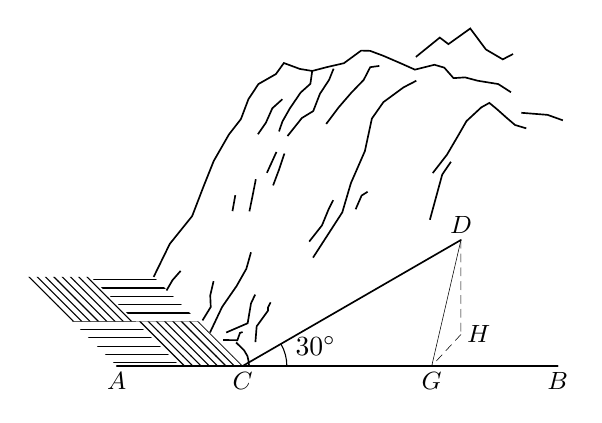
\begin{tikzpicture}[>=latex,scale=0.8,inner sep=2pt]
  \tkzDefPoints{0/0/C,-2/0/A,3/0/G,5/0/B}
  \tkzDefShiftPoint[C](30:4){D}
  \tkzDefShiftPoint[D](270:1.5){H}
  \tkzDrawSegments[semithick](A,B C,D)
  \tkzDrawSegments(D,G)
  \tkzDrawSegments[densely dashed](H,G D,H)
  \tkzLabelPoints(A,B,C,G)
  \tkzLabelPoints[above](D)
  \tkzLabelPoints[right](H)
  \tkzMarkAngle[size=0.7](G,C,D)
  \tkzLabelAngle[pos=1.2](G,C,D){\ang{30}}
  \fill[pattern=north west lines](C)--++(135:1)--++(-1,0)coordinate(E)--++(-45:1)--cycle;
  \fill[pattern=north west lines](E)--++(135:1)--++(-1,0)--++(-45:1)--cycle;
  \fill[pattern=horizontal lines](A)--++(1,0)--++(135:1)--++(-1,0)--cycle;
  \fill[pattern=horizontal lines](E)--++(1,0)--++(135:1)--++(-1,0)--cycle;
  \draw[semithick]
  (-1.414,1.414)--(-1.158,1.938)--(-0.803,2.379)--(-0.631,2.827)--(-0.460,3.255)--(-0.219,3.675)--(-0.029,3.919)--( 0.090,4.234)--( 0.249,4.475)--( 0.527,4.634)--( 0.653,4.809)--( 0.907,4.715)--( 1.103,4.683)
( 0.576,3.723)--( 0.629,3.879)--( 0.747,4.087)--( 0.919,4.340)--( 1.074,4.479)--( 1.103,4.683)--( 1.336,4.744)--( 1.606,4.806)--( 1.879,5.006)--( 2.022,5.002)--( 2.231,4.924)--( 2.525,4.797)--( 2.733,4.704)--( 3.043,4.781)--( 3.199,4.736)--( 3.346,4.569)--( 3.529,4.581)--( 3.729,4.528)--( 4.056,4.475)--( 4.258,4.345)
( 0.241,3.678)--( 0.368,3.862)--( 0.470,4.091)--( 0.629,4.234)
( 2.749,4.906)--( 3.128,5.213)--( 3.265,5.109)--( 3.612,5.357)--( 3.860,5.024)--( 4.128,4.867)--( 4.291,4.952)
( 1.116,1.720)--( 1.580,2.438)--( 1.717,2.902)--( 1.939,3.411)--( 2.050,3.927)--( 2.233,4.188)--( 2.553,4.423)--( 2.756,4.528)
( 1.325,3.842)--( 1.521,4.103)--( 1.724,4.338)--( 1.920,4.541)--( 2.024,4.743)--( 2.168,4.763)
( 0.711,3.650)--( 0.939,3.936)--( 1.119,4.046)--( 1.225,4.319)--( 1.372,4.544)--( 1.442,4.719)
( 3.016,3.062)--( 3.243,3.355)--( 3.424,3.664)--( 3.552,3.887)--( 3.787,4.105)--( 3.915,4.176)--( 4.039,4.073)--( 4.187,3.941)--( 4.323,3.825)--( 4.501,3.772)
( 4.422,4.019)--( 4.839,3.986)--( 5.082,3.899)
( 2.971,2.321)--( 3.167,3.039)--( 3.305,3.241)
(-0.520,0.531)--(-0.328,0.936)--(-0.098,1.268)--( 0.057,1.542)--( 0.131,1.804)
(-0.639,0.723)--(-0.508,0.936)--(-0.516,1.120)--(-0.463,1.346)
(-1.210,1.198)--(-1.115,1.362)--(-0.986,1.509)
(-0.262,0.531)--( 0.078,0.678)--( 0.131,0.993)--( 0.197,1.133)
( 0.201,0.379)--( 0.221,0.629)--( 0.402,0.879)--( 0.402,0.932)--( 0.443,1.010)
(-0.313,0.412)--(-0.085,0.409)--(-0.044,0.525)--(-0.002,0.538)
(-0.106,0.373)--( 0.021,0.249)--( 0.075,0.156)--( 0.091,0.083)--( 0.101,0.002)
( 1.792,2.487)--( 1.887,2.705)--( 1.982,2.765)
( 1.055,1.974)--( 1.258,2.232)--( 1.364,2.489)--( 1.436,2.631)
( 0.482,2.866)--( 0.580,3.127)--( 0.662,3.372)
( 0.384,3.066)--( 0.535,3.397)
( 0.106,2.454)--( 0.151,2.678)--( 0.208,2.964)
(-0.163,2.458)--(-0.118,2.711);
\end{tikzpicture}
\end{document}